%%%%%%%%%%%%%%%%%%%%%%%%%%%%%%%%%%%%%%%%%%%%%%%%%%%%%%%%%%%%%%%%%%%%%%%%%%%%%
% Chapter 1: Introducción 
%%%%%%%%%%%%%%%%%%%%%%%%%%%%%%%%%%%%%%%%%%%%%%%%%%%%%%%%%%%%%%%%%%%%%%%%%%%%%%%

Este capítulo servirá para explicar que es la computación evolutiva, y cuál es su propósito a la hora 

%---------------------------------------------------------------------------------
\section{Clasificación de problemas}
\label{1:sec:1}

Existen una gran cantidad de problemas que se abordan hoy en día desde el área de las matemáticas, la inteligencia artificial o la ingeniería. Muchos de estos problemas pueden tener diversas aplicaciones prácticas en ámbitos muy variados, y otros muchas veces sirven como formulaciones teóricas cuyo objetivo es encontrar cuales son los límites de la tecnología. \\

Los sistemas computacionales encargados de resolver estos problemas, pueden pensarse como \textbf{cajas negras} (\textit{black boxes}). Este esquema mental que usamos para describir los sistemas encargados de resolver problemas, parte de la base de que un sistema es una caja que recibe una serie de entradas desde el exterior, y que a partir de un modelo o programa que tiene almacenado, es capaz de procesar dicho conjunto de señales de entrada para devolver una salida. \\

El nombre \textbf{caja negra} viene dado porque normalmente, este modelo que procesa las señaeles no viene especificado de manera explícita, y por tanto puede tener diversas formas: por ejemplo puede ser una ecuación o conjunto de ecuaciones que procesen una entrada numérica, o también una herramienta estadística que devuelva una estimación a partir de la entrada, o incluso puede ser un modelo lógico que ejecute una serie de sentencias para procesar señales. \\

En cualquier caso, esta \textbf{caja negra} tiene tres partes fundamentales: las entradas, el modelo de procesamiento y la salida. Además, está claro que la parte fundamental es el modelo de computación, que de ser conocido nos permitiría calcular la salida para cualquier entrada al sistema.

\begin{figure}[ht]
    \centering
    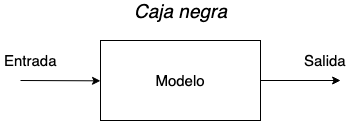
\includegraphics[scale=0.6]{mem/images/cap-1/1-1.png}
    \caption{Esquema general de un modelo computacional de caja negra}
    \label{fig:my_label}
\end{figure}

Este esquema que hemos definido es muy conveniente para establecer un criterio de clasificación de problemas, en función de que partes del sistema son conocidas y cuales no. A partir de esto podemos diferenciar en tres tipos de problemas:

\subsubsection{Optimización}
Los problemas de optimización son aquellos en los que se conoce el modelo, además de la salida que se espera, o al menos una descripción de la misma, y en función de ello, se debe calcular cuales son los valores de entrada que proporcionan dicha salida. \\

Existen multitud de problemas que se clasifican en esta categoría, aunque quizás uno de los más clásicos es el problema de viajante de comercio (\textbf{TSP}). Este problema consiste en encontrar la secuencia de rutas de coste mínimo dado un grafo de ciudades y sus interconexiones, de tal forma que cada una de las ciudades sea visitada solo una vez.\\

Como vemos, en este problema, está especificada cual es la salida esperada del problema, además del modelo de computación, sin embargo, lo que desconocemos es cual será la entrada, es decir, la combinación de rutas que minimizará el coste y que satisface las restricciones.

\subsubsection{Modelización}

En los problemas de modelización, se conocen las entradas y sus correspondientes salidas, pero se desconoce cual es el modelo de computación que debe usarse para procesarlas. \\


Este es el tipo de problemas que se abordan en áreas como el \textbf{Machine Learning}, puesto que en estos problemas se suele tener un conjunto de datos en los que existe una correspondecia entre las entradas y su resultado esperado. El problema está en crear un modelo que sea capaz de \textit{aprender} a partir de dichos datos y por tanto, sea capaz de generalizar y extraer características de datos que no haya procesado previamente.

\subsubsection{Simulación}

Este es el tipo de problemas más lineales, pues en ellos se conoce cuales serán las entradas y el modelo de computación, pero se desconoce cual será la salida. \\

Existen multitud de ejemplos de problemas de simulación, como por ejemplo; simulación de fluidos, meteorológica o económica. Este tipo de problemas tienen una gran utilidad, pues nos permiten predecir una realidad futura, lo cual es crucial en múltiples ámbitos. \\

%------

Otra clasificación posible que se puede hacer de los problemas es en función de la \textit{complejidad} que entraña resolverlos. La complejidad de un problema es la complejidad computacional del mejor algoritmo que lo resuelve. \\


%---------------------------------------------------------------------------------
\section{Computación evolutiva}
\label{1:sec:2}

¿Que es la computación evolutiva?

%---------------------------------------------------------------------------------
\section{Algoritmos evolutivos}
\label{1:sec:3}

Que es una algoritmo evolutivo

Bla, bla, bla  \ref{1:sec:1}

%---------------------------------------------------------------------------------
\section{CLasificación}
\label{1:sec:4}

Cual es la clasificación de los algoritmos evolutivos.
